\documentclass{article}

\usepackage[bottom=1cm, right=1cm, left=1cm, top=1cm]{geometry}
\pagenumbering{gobble}

\usepackage{multirow}
\usepackage{makecell}

\usepackage{musixtex}
\usepackage{gtabs}
\usepackage{tikz}

\newcommand*{\musicintext}[1]{
    \let\extractline\relax
    \nobarnumbers\staffbotmarg0pt
    \startextract\addspace{-\afterruleskip}\qsk
    \staffbotmarg2\Interligne\Notes#1\en
    \endextract
}

\setchordscheme{
    rotate = -90,
    restrict-bounding-box = true,
    x-unit=1.75mm,
    y-unit=2.75mm,
    line-width = 0.4pt,
    finger-radius = .5,
    muted-style = {cross out, draw, scale = 0.65}
}

\begin{document}

\setlength\tabcolsep{0pt}

\begin{center}
\begin{tabular}{ p{2.3cm} p{1.1cm} p{4.6cm} p{2.1cm} p{4.5cm} p{1.7cm} p{3.2cm} }
    \multicolumn{7}{c}{
        \Huge{Jazz Chords in C}
    } \\
    \hline
    \makecell[cl]{
        \textcolor{blue}{Minor} \\
        \textcolor{blue}{Seventh}
    } &
    \makecell[cl]{
        Cmin\textsuperscript{7} \\
        Cm\textsuperscript{7} \\
        C\textminus\textsuperscript{7}
    } &
    \makecell[cc]{
        \raisebox{-0.4\normalbaselineskip}[0pt][0pt]{
            \begin{tabular}{ *{6}{p{0.7cm}} }
                \makecell[cc]{1} &
                \makecell[cc]{m3} &
                \makecell[cc]{5} &
                \makecell[cc]{m7} & & \\
                \makecell[cc]{\textbf{C}} &
                \makecell[cc]{\textbf{E\textsuperscript{$\flat$}}} &
                \makecell[cc]{\textbf{G}} &
                \makecell[cc]{\textbf{B\textsuperscript{$\flat$}}} & & \\
                \multicolumn{3}{ c }{
                    \raisebox{0.9\normalbaselineskip}[0pt][0pt]{
                        $\underbrace{\hspace*{1.6cm}}$
                    }
                } & & & \\
                \multicolumn{3}{ c }{
                    \raisebox{0.8\normalbaselineskip}[0pt][0pt]{
                        \footnotesize{Minor Triad}
                    }
                } & & & \\
            \end{tabular}
        }
    } &
    \makecell[cc]{
        \raisebox{0ex}[5ex][0ex]{
            \musicintext{\zw{c}\accshift=0.6mm\zw{_e}\accshift=0mm\zw{g}\zw{_i}}
        }
    } &
    \makecell[cc]{
        \begin{tikzpicture}
            \node{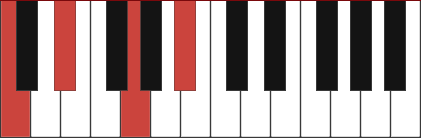
\includegraphics[width=0.2\textwidth]{assets/cm7.png}};
        \end{tikzpicture}
    } &
    \makecell[cc]{
        \raisebox{2mm}{
            \chordscheme[
                position = 3,
                barre = 1/1-5,
                finger = 2/2,
                finger = 3/4,
                mute = 6
            ]
        }
    } & \\
    \hline
    \makecell[cl]{
        \textcolor{red}{Dominant} \\
        \textcolor{red}{Seventh}
    } &
    \makecell[cl]{
        C\textsuperscript{7}
    } &
    \makecell[cc]{
        \raisebox{-0.4\normalbaselineskip}[0pt][0pt]{
            \begin{tabular}{ *{6}{p{0.7cm}} }
                \makecell[cc]{1} &
                \makecell[cc]{M3} &
                \makecell[cc]{5} &
                \makecell[cc]{m7} & & \\
                \makecell[cc]{\textbf{C}} &
                \makecell[cc]{\textbf{E}} &
                \makecell[cc]{\textbf{G}} &
                \makecell[cc]{\textbf{B\textsuperscript{$\flat$}}} & & \\
                \multicolumn{3}{ c }{
                    \raisebox{0.9\normalbaselineskip}[0pt][0pt]{
                        $\underbrace{\hspace*{1.6cm}}$
                    }
                } & & & \\
                \multicolumn{3}{ c }{
                    \raisebox{0.8\normalbaselineskip}[0pt][0pt]{
                        \footnotesize{Major Triad}
                    }
                } & & & \\
            \end{tabular}
        }
    } &
    \makecell[cc]{
        \raisebox{0ex}[5ex][0ex]{
            \musicintext{\zw{c}\zw{e}\zw{g}\zw{_i}}
        }
    } &
    \makecell[cc]{
        \begin{tikzpicture}
            \node{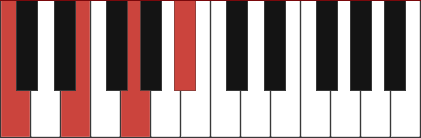
\includegraphics[width=0.2\textwidth]{assets/c7.png}};
        \end{tikzpicture}} &
    \makecell[cc]{
        \raisebox{2mm}{
            \chordscheme[
                finger = 1/2,
                finger = 3/3,
                finger = 2/4,
                finger = 3/5,
                mute = 6,
                ring = 1
            ]
        }
    } &
    \makecell[cl]{
        \footnotesize{C\textsuperscript{7\textminus5}: dim 5\textsuperscript{th}} \\
        \footnotesize{C\textsuperscript{7+5}: aug 5\textsuperscript{th}}
    } \\
    \hline
    \makecell[cl]{
        \textcolor[RGB]{0,150,20}{Major} \\
        \textcolor[RGB]{0,150,20}{Seventh}
    } &
    \makecell[cl]{
        Cmaj\textsuperscript{7} \\
        CM\textsuperscript{7} \\
        C$\Delta$\textsuperscript{7}
    } &
    \makecell[cc]{
        \raisebox{-0.4\normalbaselineskip}[0pt][0pt]{
            \begin{tabular}{ *{6}{p{0.7cm}} }
                \makecell[cc]{1} &
                \makecell[cc]{M3} &
                \makecell[cc]{5} &
                \makecell[cc]{M7} & & \\
                \makecell[cc]{\textbf{C}} &
                \makecell[cc]{\textbf{E}} &
                \makecell[cc]{\textbf{G}} &
                \makecell[cc]{\textbf{B}} & & \\
                \multicolumn{3}{ c }{
                    \raisebox{0.9\normalbaselineskip}[0pt][0pt]{
                        $\underbrace{\hspace*{1.6cm}}$
                    }
                } & & & \\
                \multicolumn{3}{ c }{
                    \raisebox{0.8\normalbaselineskip}[0pt][0pt]{
                        \footnotesize{Major Triad}
                    }
                } & & & \\
            \end{tabular}
        }
    } &
    \makecell[cc]{
        \raisebox{0ex}[5ex][0ex]{
            \musicintext{\zw{c}\zw{e}\zw{g}\zw{i}}
        }
    } &
    \makecell[cc]{
        \begin{tikzpicture}
            \node{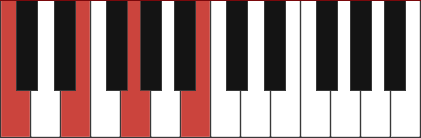
\includegraphics[width=0.2\textwidth]{assets/cmaj7.png}};
        \end{tikzpicture}
    } &
    \makecell[cc]{
        \raisebox{2mm}{
            \chordscheme[
                finger = 2/4,
                finger = 3/5,
                mute = 6,
                ring = {1,2,3}
            ]
        }
    } & \\
    \hline
    \makecell[cl]{
        Major \\
        Sixth
    } &
    \makecell[cl]{
        C\textsuperscript{6}
    } &
    \makecell[cc]{
        \raisebox{-0.4\normalbaselineskip}[0pt][0pt]{
            \begin{tabular}{ *{6}{p{0.7cm}} }
                \makecell[cc]{1} &
                \makecell[cc]{M3} &
                \makecell[cc]{5} &
                \makecell[cc]{M6} & & \\
                \makecell[cc]{\textbf{C}} &
                \makecell[cc]{\textbf{E}} &
                \makecell[cc]{\textbf{G}} &
                \makecell[cc]{\textbf{D}} & & \\
                \multicolumn{3}{ c }{
                    \raisebox{0.9\normalbaselineskip}[0pt][0pt]{
                        $\underbrace{\hspace*{1.6cm}}$
                    }
                } & & & \\
                \multicolumn{3}{ c }{
                    \raisebox{0.8\normalbaselineskip}[0pt][0pt]{
                        \footnotesize{Major Triad}
                    }
                } & & & \\
            \end{tabular}
        }
    } &
    \makecell[cc]{
        \raisebox{0ex}[5ex][0ex]{
            \musicintext{\zw{c}\zw{e}\zw{g}\qsk\zw{h}}
        }
    } &
    \makecell[cc]{
        \begin{tikzpicture}
            \node{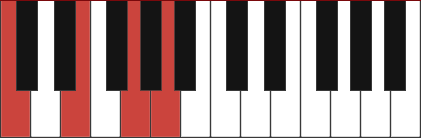
\includegraphics[width=0.2\textwidth]{assets/c6.png}};
        \end{tikzpicture}
    } &
    \makecell[cc]{
        \raisebox{2mm}{
            \chordscheme[
                finger = 1/2,
                finger = 2/3,
                finger = 2/4,
                finger = 3/5,
                mute = 6,
                ring = 1
            ]
        }
    } &
    \makecell[cl]{
        \footnotesize{Cm\textsuperscript{6}: dim 3\textsuperscript{rd}} \\
        \footnotesize{C\textsuperscript{6/9}: add 9\textsuperscript{th}}
    } \\
    \hline
    \makecell[cl]{
        \textcolor{orange}{Diminished}
    } &
    \makecell[cl]{
        C\textsuperscript{o} \\
        Cdim
    } &
    \makecell[cc]{
        \begin{tabular}{ *{6}{p{0.7cm}} }
            \makecell[cc]{1} &
            \makecell[cc]{m3} &
            \makecell[cc]{d5} & & & \\
            \makecell[cc]{\textbf{C}} &
            \makecell[cc]{\textbf{E\textsuperscript{$\flat$}}} &
            \makecell[cc]{\textbf{G\textsuperscript{$\sharp$}}} & & & \\
        \end{tabular}
    } &
    \makecell[cc]{
        \raisebox{0ex}[5ex][0ex]{
            \musicintext{\hqsk\zw{c}\accshift=1.4mm\zw{_e}\accshift=0mm\zw{_g}}
        }
    } &
    \makecell[cc]{
        \begin{tikzpicture}
            \node{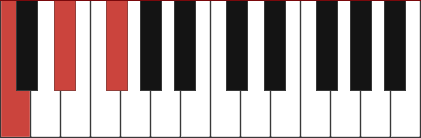
\includegraphics[width=0.2\textwidth]{assets/cdim.png}};
        \end{tikzpicture}
    } &
    \makecell[cc]{
        \raisebox{2mm}{
            \chordscheme[
                position = 3,
                finger = 2/2,
                finger = 3/3,
                finger = 2/4,
                finger = 1/5,
                mute = {1,6}
            ]
        }
    } &
    \makecell[cl]{
        \footnotesize{interchangable with C\textsuperscript{o7}}
    } \\
    \hline
    \makecell[cl]{
        Fully \\
        Diminished \\
        Seventh
    } &
    \makecell[cl]{
        C\textsuperscript{o7} \\
        Cdim\textsuperscript{7}
    } &
    \makecell[cc]{
        \raisebox{-0.4\normalbaselineskip}[0pt][0pt]{
            \begin{tabular}{ *{6}{p{0.7cm}} }
                \makecell[cc]{1} &
                \makecell[cc]{m3} &
                \makecell[cc]{d5} &
                \makecell[cc]{d7} & & \\
                \makecell[cc]{\textbf{C}} &
                \makecell[cc]{\textbf{E\textsuperscript{$\flat$}}} &
                \makecell[cc]{\textbf{G\textsuperscript{$\flat$}}} &
                \makecell[cc]{\textbf{B\textsuperscript{$\flat\flat$}}} & & \\
                \multicolumn{3}{ c }{
                    \raisebox{0.9\normalbaselineskip}[0pt][0pt]{
                        $\underbrace{\hspace*{1.6cm}}$
                    }
                } & & & \\
                \multicolumn{3}{ c }{
                    \raisebox{0.8\normalbaselineskip}[0pt][0pt]{
                        \footnotesize{\textcolor{orange}{Diminished}}
                    }
                } & & & \\
            \end{tabular}
        }
    } &
    \makecell[cc]{
        \raisebox{0ex}[5ex][0ex]{
            \musicintext{\qsk\zw{c}\accshift=0.4mm\zw{_e}\accshift=2.8mm\zw{_g}\accshift=0mm\zw{<i}}
        }
    } &
    \makecell[cc]{
        \begin{tikzpicture}
            \node{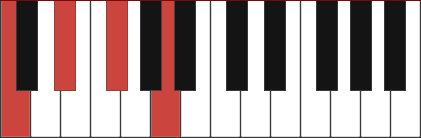
\includegraphics[width=0.2\textwidth]{assets/cdim7.png}};
        \end{tikzpicture}
    } &
    \makecell[cc]{
        \raisebox{2mm}{
            \chordscheme[
                position = 7,
                finger = 2/3,
                finger = 1/4,
                finger = 3/5,
                finger = 2/6,
                mute = {1,2},
            ]
        }
    } &
    \makecell[cl]{
        \footnotesize{interchangable with C\textsuperscript{o}}
    } \\
    \hline
    \makecell[cl]{
        Half \\
        Diminished \\
        Seventh
    } &
    \makecell[cl]{
        C\textsuperscript{\o{}7} \\
        Cm\textsuperscript{7$\flat$5} \\
        C\textminus\textsuperscript{7$\flat$5}
    } &
    \makecell[cc]{
        \raisebox{-0.4\normalbaselineskip}[0pt][0pt]{
            \begin{tabular}{ *{6}{p{0.7cm}} }
                \makecell[cc]{1} &
                \makecell[cc]{m3} &
                \makecell[cc]{d5} &
                \makecell[cc]{m7} & & \\
                \makecell[cc]{\textbf{C}} &
                \makecell[cc]{\textbf{E\textsuperscript{$\flat$}}} &
                \makecell[cc]{\textbf{G\textsuperscript{$\flat$}}} &
                \makecell[cc]{\textbf{B\textsuperscript{$\flat$}}} & & \\
                \multicolumn{3}{ c }{
                    \raisebox{0.9\normalbaselineskip}[0pt][0pt]{
                        $\underbrace{\hspace*{1.6cm}}$
                    }
                } & & & \\
                \multicolumn{3}{ c }{
                    \raisebox{0.8\normalbaselineskip}[0pt][0pt]{
                        \footnotesize{\textcolor{orange}{Diminished}}
                    }
                } & & & \\
            \end{tabular}
        }
    } &
    \makecell[cc]{
        \raisebox{0ex}[5ex][0ex]{
            \musicintext{\tqsk\zw{c}\accshift=0.4mm\zw{_e}\accshift=2.2mm\zw{_g}\accshift=0mm\zw{_i}}
        }
    } &
    \makecell[cc]{
        \begin{tikzpicture}
            \node{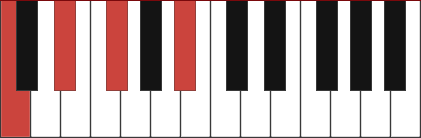
\includegraphics[width=0.2\textwidth]{assets/cm7b5.png}};
        \end{tikzpicture}
    } &
    \makecell[cc]{
        \raisebox{2mm}{
            \chordscheme[
                position = 3,
                barre = 1/3-5,
                finger = 4/1,
                finger = 2/2,
                finger = 2/4,
                mute = 6
            ]
        }
    } &
    \makecell[cl]{
        \footnotesize{can also be thought of} \\
        \footnotesize{as Cm\textsuperscript{7} with a dim 5\textsuperscript{th}}
    } \\
    \hline
    \makecell[cl]{
        Minor \\
        Ninth
    } &
    \makecell[cl]{
        Cm\textsuperscript{9}
    } &
    \makecell[cc]{
        \raisebox{-0.4\normalbaselineskip}[0pt][0pt]{
            \begin{tabular}{ *{6}{p{0.7cm}} }
                \makecell[cc]{1} &
                \makecell[cc]{m3} &
                \makecell[cc]{5} &
                \makecell[cc]{m7} &
                \makecell[cc]{M9} & \\
                \makecell[cc]{\textbf{C}} &
                \makecell[cc]{\textbf{E\textsuperscript{$\flat$}}} &
                \makecell[cc]{\textbf{G}} &
                \makecell[cc]{\textbf{B\textsuperscript{$\flat$}}} &
                \makecell[cc]{\textbf{D}} & \\
                \multicolumn{4}{ c }{
                    \raisebox{0.9\normalbaselineskip}[0pt][0pt]{
                        $\underbrace{\hspace*{2.3cm}}$
                    }
                } & & \\
                \multicolumn{4}{ c }{
                    \raisebox{0.8\normalbaselineskip}[0pt][0pt]{
                        \footnotesize{\textcolor{blue}{Minor Seventh}}
                    }
                } & & \\
            \end{tabular}
        }
    } &
    \makecell[cc]{
        \raisebox{0ex}[5ex][0ex]{
            \musicintext{\zw{c}\accshift=0.6mm\zw{_e}\accshift=0mm\zw{g}\zw{_i}\zw{k}}
        }
    } &
    \makecell[cc]{
        \begin{tikzpicture}
            \node{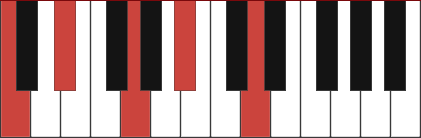
\includegraphics[width=0.2\textwidth]{assets/cm9.png}};
        \end{tikzpicture}} &
    \makecell[cc]{
        \raisebox{2mm}{
            \chordscheme[
                position = 6,
                finger = 2/3,
                finger = 3/4,
                finger = 1/5,
                finger = 3/6,
                mute = {1,2}
            ]
        }
    } & \\
    \hline
    \makecell[cl]{
        \textcolor[RGB]{80,0,150}{Dominant} \\
        \textcolor[RGB]{80,0,150}{Ninth}
    } &
    \makecell[cl]{
        C\textsuperscript{9}
    } &
    \makecell[cc]{
        \raisebox{-0.4\normalbaselineskip}[0pt][0pt]{
            \begin{tabular}{ *{6}{p{0.7cm}} }
                \makecell[cc]{1} &
                \makecell[cc]{M3} &
                \makecell[cc]{5} &
                \makecell[cc]{m7} &
                \makecell[cc]{M9} & \\
                \makecell[cc]{\textbf{C}} &
                \makecell[cc]{\textbf{E}} &
                \makecell[cc]{\textbf{G}} &
                \makecell[cc]{\textbf{B\textsuperscript{$\flat$}}} &
                \makecell[cc]{\textbf{D}} & \\
                \multicolumn{4}{ c }{
                    \raisebox{0.9\normalbaselineskip}[0pt][0pt]{
                        $\underbrace{\hspace*{2.3cm}}$
                    }
                } & & \\
                \multicolumn{4}{ c }{
                    \raisebox{0.8\normalbaselineskip}[0pt][0pt]{
                        \footnotesize{\textcolor{red}{Dominant Seventh}}
                    }
                } & & \\
            \end{tabular}
        }
    } &
    \makecell[cc]{
        \raisebox{0ex}[5ex][0ex]{
            \musicintext{\zw{c}\zw{e}\zw{g}\zw{_i}\zw{k}}
        }
    } &
    \makecell[cc]{
        \begin{tikzpicture}
            \node{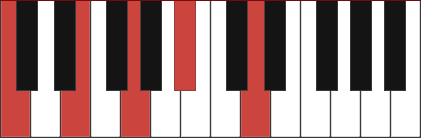
\includegraphics[width=0.2\textwidth]{assets/c9.png}};
        \end{tikzpicture}
    } &
    \makecell[cc]{
        \raisebox{2mm}{
            \chordscheme[
                finger = 3/2,
                finger = 3/3,
                finger = 2/4,
                finger = 3/5,
                mute = 6,
                ring = 1
            ]
        }
    } &
    \makecell[cl]{
        \footnotesize{opt. 5\textsuperscript{th}}
    } \\
    \hline
    \makecell[cl]{
        Major \\
        Ninth
    } &
    \makecell[cl]{
        Cmaj\textsuperscript{9}
    } &
    \makecell[cc]{
        \raisebox{-0.4\normalbaselineskip}[0pt][0pt]{
            \begin{tabular}{ *{6}{p{0.7cm}} }
                \makecell[cc]{1} &
                \makecell[cc]{M3} &
                \makecell[cc]{5} &
                \makecell[cc]{M7} &
                \makecell[cc]{M9} & \\
                \makecell[cc]{\textbf{C}} &
                \makecell[cc]{\textbf{E}} &
                \makecell[cc]{\textbf{G}} &
                \makecell[cc]{\textbf{B}} &
                \makecell[cc]{\textbf{D}} & \\
                \multicolumn{4}{ c }{
                    \raisebox{0.9\normalbaselineskip}[0pt][0pt]{
                        $\underbrace{\hspace*{2.3cm}}$
                    }
                } & & \\
                \multicolumn{4}{ c }{
                    \raisebox{0.8\normalbaselineskip}[0pt][0pt]{
                        \footnotesize{\textcolor[RGB]{0,150,20}{Major Seventh}}
                    }
                } & & \\
            \end{tabular}
        }
    } &
    \makecell[cc]{
        \raisebox{0ex}[5ex][0ex]{
            \musicintext{\zw{c}\zw{e}\zw{g}\zw{i}\zw{k}}
        }
    } &
    \makecell[cc]{
        \begin{tikzpicture}
            \node{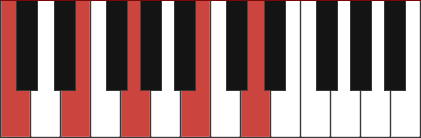
\includegraphics[width=0.2\textwidth]{assets/cmaj9.png}};
        \end{tikzpicture}
    } &
    \makecell[cc]{
        \raisebox{2mm}{
            \chordscheme[
                finger = 3/2,
                finger = 4/3,
                finger = 2/4,
                finger = 3/5,
                mute = {1,6}
            ]
        }
    } & \\
    \hline
    \makecell[cl]{
        Eleventh
    } &
    \makecell[cl]{
        C\textsuperscript{11}
    } &
    \makecell[cc]{
        \raisebox{-0.4\normalbaselineskip}[0pt][0pt]{
            \begin{tabular}{ *{6}{p{0.7cm}} }
                \makecell[cc]{1} &
                \makecell[cc]{5} &
                \makecell[cc]{m7} &
                \makecell[cc]{M9} &
                \makecell[cc]{11} & \\
                \makecell[cc]{\textbf{C}} &
                \makecell[cc]{\textbf{G}} &
                \makecell[cc]{\textbf{B\textsuperscript{$\flat$}}} &
                \makecell[cc]{\textbf{D}} &
                \makecell[cc]{\textbf{F}} & \\
                \multicolumn{4}{ c }{
                    \raisebox{0.9\normalbaselineskip}[0pt][0pt]{
                        $\underbrace{\hspace*{2.3cm}}$
                    }
                } & & \\
                \multicolumn{4}{ c }{
                    \raisebox{0.8\normalbaselineskip}[0pt][0pt]{
                        \footnotesize{\textcolor[RGB]{80,0,150}{Dominant Ninth}}
                    }
                } & & \\
            \end{tabular}
        }
    } &
    \makecell[cc]{
        \raisebox{0ex}[5ex][0ex]{
            \musicintext{\zw{c}\zw{g}\zw{_i}\zw{k}\zw{m}}
        }
    } &
    \makecell[cc]{
        \begin{tikzpicture}
            \node{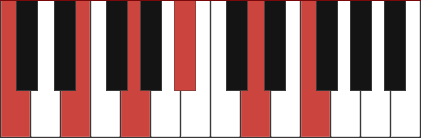
\includegraphics[width=0.2\textwidth]{assets/c11.png}};
        \end{tikzpicture}
    } &
    \makecell[cc]{
        \raisebox{2mm}{
            \chordscheme[
                barre = 3/1-5,
                mute = 6
            ]
        }
    } &
    \makecell[cl]{
        \footnotesize{omit 3\textsuperscript{rd}} \\
        \footnotesize{optional 1\textsuperscript{st}, 5\textsuperscript{th}, 9\textsuperscript{th}}
    } \\
    \hline
    \makecell[cl]{
        Thirteenth
    } &
    \makecell[cl]{
        C\textsuperscript{13}
    } &
    \makecell[cc]{
        \raisebox{-0.4\normalbaselineskip}[0pt][0pt]{
            \begin{tabular}{ *{6}{p{0.7cm}} }
                \makecell[cc]{1} &
                \makecell[cc]{M3} &
                \makecell[cc]{5} &
                \makecell[cc]{m7} &
                \makecell[cc]{M9} &
                \makecell[cc]{M13} \\
                \makecell[cc]{\textbf{C}} &
                \makecell[cc]{\textbf{E}} &
                \makecell[cc]{\textbf{G}} &
                \makecell[cc]{\textbf{B\textsuperscript{$\flat$}}} &
                \makecell[cc]{\textbf{D}} &
                \makecell[cc]{\textbf{A}} \\
                \multicolumn{5}{ c }{
                    \raisebox{0.9\normalbaselineskip}[0pt][0pt]{
                        $\underbrace{\hspace*{3cm}}$
                    }
                } & \\
                \multicolumn{5}{ c }{
                    \raisebox{0.8\normalbaselineskip}[0pt][0pt]{
                        \footnotesize{\textcolor[RGB]{80,0,150}{Dominant Ninth}}
                    }
                } & \\
            \end{tabular}
        }
    } &
    \makecell[cc]{
        \raisebox{0ex}[5ex][0ex]{
            \musicintext{\zw{c}\zw{e}\zw{g}\zw{_i}\zw{k}\zw{o}}
        }
    } &
    \makecell[cc]{
        \begin{tikzpicture}
            \node{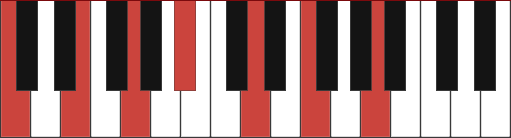
\includegraphics[width=0.2\textwidth]{assets/c13.png}};
        \end{tikzpicture}
    } &
    \makecell[cc]{
        \raisebox{2mm}{
            \chordscheme[
                position = 8,
                finger = 3/2,
                finger = 2/3,
                finger = 1/4,
                finger = 1/6,
                mute = {1,5}
            ]
        }
    } &
    \makecell[cl]{
        \footnotesize{optional 1\textsuperscript{st}, 5\textsuperscript{th}, 9\textsuperscript{th}}
    } \\
    \hline
    \makecell[cl]{
        Augmented
    } &
    \makecell[cl]{
        C\textsuperscript{+} \\
        Caug \\
        C\textsuperscript{$\sharp$5}
    } &
    \makecell[cc]{
        \begin{tabular}{ *{6}{p{0.7cm}} }
            \makecell[cc]{1} &
            \makecell[cc]{M3} &
            \makecell[cc]{d5} & & & \\
            \makecell[cc]{\textbf{C}} &
            \makecell[cc]{\textbf{E}} &
            \makecell[cc]{\textbf{G\textsuperscript{$\sharp$}}} & & & \\
        \end{tabular}
    } &
    \makecell[cc]{
        \raisebox{0ex}[5ex][0ex]{
            \musicintext{\zw{c}\zw{e}\zw{^g}}
        }
    } &
    \makecell[cc]{
        \begin{tikzpicture}
            \node{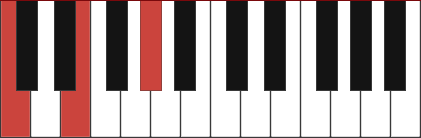
\includegraphics[width=0.2\textwidth]{assets/caug.png}};
        \end{tikzpicture}
    } &
    \makecell[cc]{
        \raisebox{2mm}{
            \chordscheme[
                finger = 1/2,
                finger = 1/3,
                finger = 2/4,
                finger = 3/5,
                mute = 6,
                ring = 1
            ]
        }
    } &
    \makecell[cl]{
        \footnotesize{Caug\textsuperscript{7} is identical to} \\
        \footnotesize{C\textsuperscript{7+5}}
    } \\
    \hline
    \makecell[cl]{
        Suspended
    } &
    \makecell[cl]{
        Csus2
    } &
    \makecell[cc]{
        \begin{tabular}{ *{6}{p{0.7cm}} }
            \makecell[cc]{1} &
            \makecell[cc]{M2} &
            \makecell[cc]{5} & & & \\
            \makecell[cc]{\textbf{C}} &
            \makecell[cc]{\textbf{D}} &
            \makecell[cc]{\textbf{G}} & & & \\
        \end{tabular}
    } &
    \makecell[cc]{
        \raisebox{0ex}[5ex][0ex]{
            \musicintext{\zw{c}\zw{g}\qsk\zw{d}}
        }
    } &
    \makecell[cc]{
        \begin{tikzpicture}
            \node{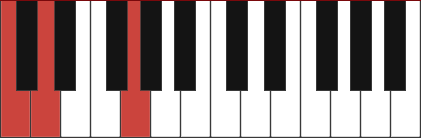
\includegraphics[width=0.2\textwidth]{assets/csus2.png}};
        \end{tikzpicture}
    } &
    \makecell[cc]{
        \raisebox{2mm}{
            \chordscheme[
                finger = 3/1,
                finger = 3/2,
                finger = 3/5,
                mute = 6,
                ring = {3,4}
            ]
        }
    } & \\
    \hline
    \makecell[cl]{
        Suspended
    } &
    \makecell[cl]{
        Csus4
    } &
    \makecell[cc]{
        \begin{tabular}{ *{6}{p{0.7cm}} }
            \makecell[cc]{1} &
            \makecell[cc]{4} &
            \makecell[cc]{5} & & & \\
            \makecell[cc]{\textbf{C}} &
            \makecell[cc]{\textbf{F}} &
            \makecell[cc]{\textbf{G}} & & & \\
        \end{tabular}
    } &
    \makecell[cc]{
        \raisebox{0ex}[5ex][0ex]{
            \musicintext{\zw{c}\zw{f}\qsk\zw{g}}
        }
    } &
    \makecell[cc]{
        \begin{tikzpicture}
            \node{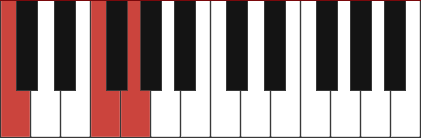
\includegraphics[width=0.2\textwidth]{assets/csus4.png}};
        \end{tikzpicture}
    } &
    \makecell[cc]{
        \raisebox{2mm}{
            \chordscheme[
                barre = 1/1-2,
                finger = 3/4,
                finger = 3/5,
                mute = 6,
                ring = 3
            ]
        }
    } & \\
    \hline
\end{tabular}
\end{center}

\bigskip

\begin{center}
    \Large Other Info
\end{center}

\normalsize

"Slash" chords: the use of the slash in chord writing simply means that whatever is below the slash must be the bass note. Consequently, C/E indicates a C major triad with an E in the bass (first inversion). Be aware that there need not be a harmonic relationship between the chord above the slash and the note below it. This makes it possible to write chords that would be impossible to analyze in Roman numerals such as Cm/F$\sharp$.

A special situation arises when a minor seventh chord is placed in first inversion (for example: Am\textsuperscript{7}/C). While this notation will agree with traditional Roman numeral analysis, it will only rarely appear in jazz chord symbols. This type of chord would almost always be written as C\textsuperscript{6}; that is, a C major chord, with an added 6\textsuperscript{th} scale degree.

In Jazz, most chords are voiced with four pitches (regardless of the chord) and are played in the left hand near middle C. This sometimes means leaving out pitches and sometimes means adding pitches (triads are rare in jazz). See a chord glossary for specifics. The right hand would either play the tune, play a solo, or emphasize roots and 5ths.

\end{document}